\chapter{Results}
\label{sec:results}

Comparing the lineplot of page views from 2009 as shown in the paper by Yasseri et al. (Figure 1) to the lineplot recreated in Figure \ref{fig:figure1} of this report, it is evident that the two lineplots exhibit close similarity. The peak in page views aligns with the date of the 2009 European Parliament Elections, indicating a clear correlation between the election and the increased interest in related Wikipedia articles. 

\begin{figure*}[t!]
    \centering
    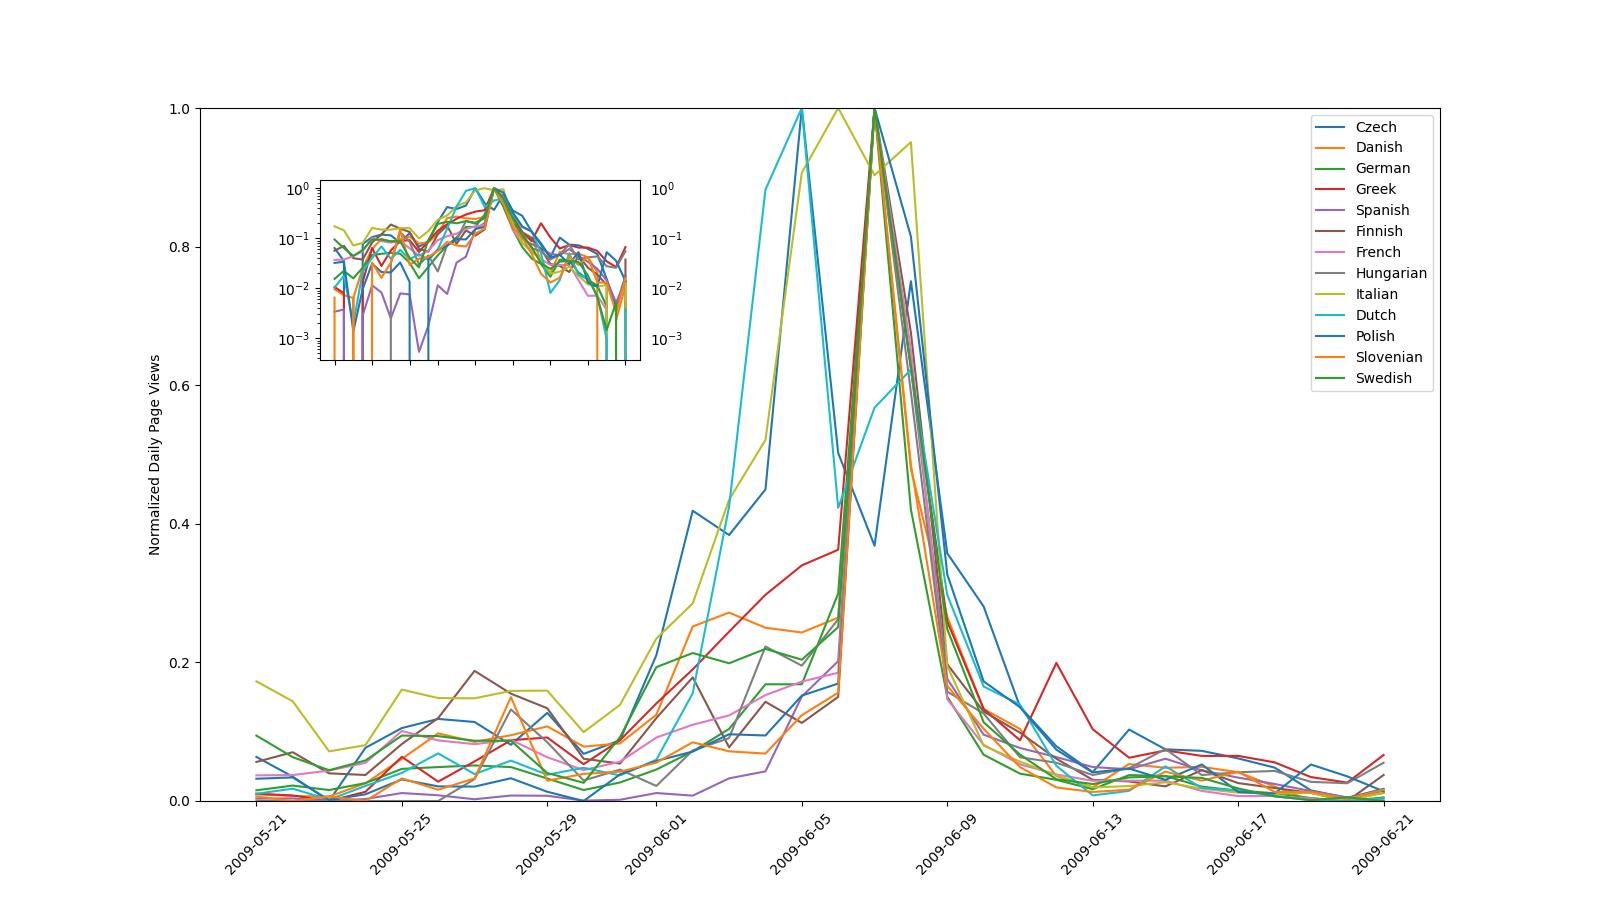
\includegraphics[width=\textwidth]{fig/lineplot_2009.png}
    \caption{'Normalized Wikipedia Election Page Views two weeks before and after the 2009 European Parliament Elections'}
    \label{fig:figure1}
\end{figure*} 
However, when visualizing the data from 2014 and 2019 in the same way, it becomes apparent that the patterns differ from those observed in the 2009 data. The peaks and fluctuations in page views do not align as closely with the election dates in these years. 
\begin{figure*}[t!]
    \centering
    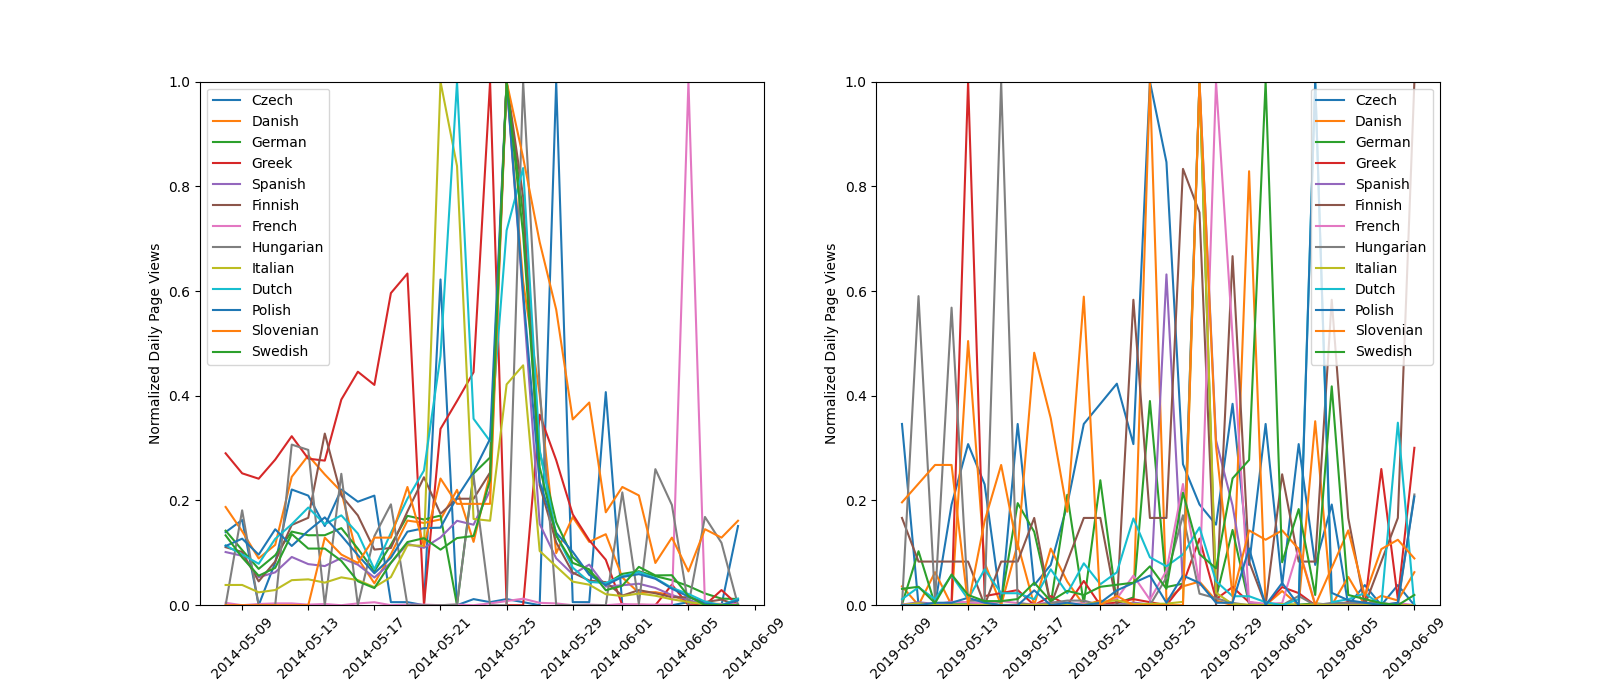
\includegraphics[width=\textwidth]{fig/lineplot_2014_2019.png}
    \caption{'Normalized Wikipedia Election Page Views two weeks before and after the 2014 (left) and 2019 (right) European Parliament Elections'}
    \label{fig:figure2}
\end{figure*}
Taking a closer look at absolute values of France, a country  where the peak does not correspond to the election date, it becomes apparent that there must be errors in the data or its retrieval, as page views are at 0 or below 10 before a seemingly random peak at around the 5th of June. Further analysis has to be performed under the assumption that the data is erroneous.
